
\section{Methodology} \label{sec:methodology}

\textcolor{black}{
UAV aerial image segmentation presents unique challenges compared with ground-level imagery, as target objects often appear at arbitrary orientations due to the aerial imaging perspective. Conventional convolution operators are sensitive to such orientation variations, which can lead to degraded segmentation accuracy. The methodology presented in this section introduces a series of convolution formulations that are specifically designed as drop-in replacements for standard convolution layers in semantic segmentation networks.These operators form the computational backbone of the proposed UAV segmentation framework, enabling rotation-aware feature extraction while maintaining efficiency suitable for large-scale aerial imagery. Their practical effectiveness is demonstrated through integration into a U-Net architecture and validated in the experimental section.
}


\subsection{Single orientation convolution formulation}
In the single-orientation case, the operation reduces to standard convolution because only one fixed kernel orientation is applied and no orientation-dependent processing is required. In standard convolution, each filter element is multiplied by its overlapping input element, and the resulting products are summed to produce the output value at the corresponding spatial location, as illustrated in Fig.~\ref{fig:standardConv}(a). Alternatively, as demonstrated in our previous work~\cite{manduhu2025airbornesensedetectdrones}, convolution can also be performed using a scatter-based approach (which we employed to implement sparse convolution). In this approach, each input pixel is multiplied by different kernel elements, and the resulting values are added to their corresponding neighboring output positions, as shown in Fig.~\ref{fig:standardConv}(b). This distributes computation across output locations rather than accumulating it at a single pixel, enabling convolution without data lowering while benefiting from the high-throughput matrix multiplication capabilities of modern GPUs. In this paper, we extend the scatter-based approach to support dense convolution.

\begin{figure}[h]
\centering
    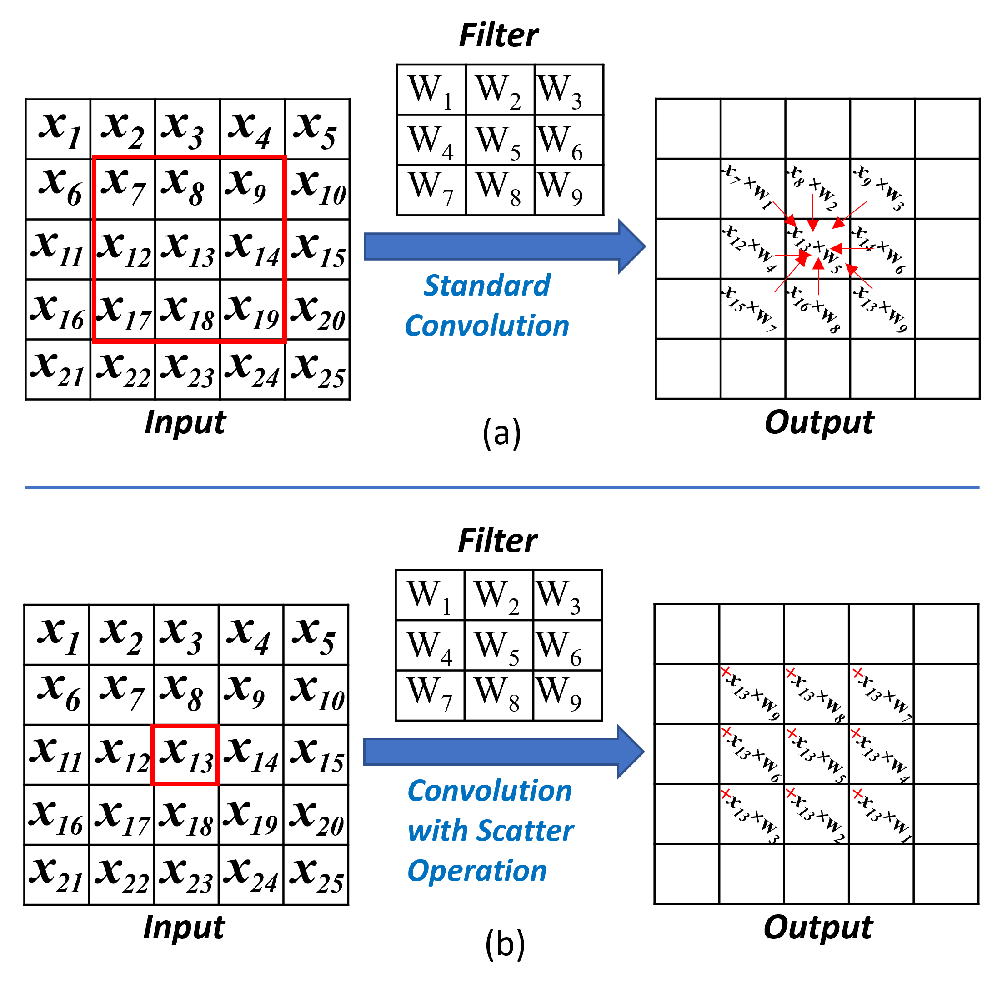
\includegraphics[width=8.5cm]{fig/method/standar-vs-scatter.pdf}
\caption{(a) Standard convolution where $x_i, w_i, y_i$ represent input, filter and output, respectively. \textcolor{black}{(b) Convolution with scatter operation where each input element is multiplied by each filter element and the results are added with those of neighboring elements.} }
\label{fig:standardConv}
\end{figure} 

Let the input be 
$\mathbf{X} \in \mathbb{R}^{C_{\mathrm{in}} \times H \times W}$ 
and the filters 
$\mathbf{W} \in \mathbb{R}^{C_{\mathrm{out}} \times C_{\mathrm{in}} \times K_h \times K_w}$, where 
$C_{\mathrm{in}}$ and $C_{\mathrm{out}}$ denote the numbers of input channels and output
channels, respectively, and 
$H$ and $W$ represent the height and width of the input feature map,
while $K_h$ and $K_w$ denote the kernel height and width.
For valid convolution, the output spatial size is
\[
H' = H - K_h + 1,
\qquad
W' = W - K_w + 1.
\]
The convolution output is
\begin{equation}
\begin{split}
Y_{c_{o},h,w}
=
\sum_{c_i=0}^{C_{\mathrm{in}}-1}
\sum_{i=0}^{K_h-1}
\sum_{j=0}^{K_w-1}
W_{c_o,c_i,i,j}\;
X_{c_i,\,h+i,\,w+j}, \\
h  \in \{0,...,H'-1\}\\
w  \in \{0,...,W'-1\}\\
c_o  \in \{0,...,C_{out}-1\}
\end{split}
\end{equation}
which is the standard sliding-window inner product formulation.
To convert convolution into matrix multiplication, every 
$K_h \times K_w$ receptive field from $\mathbf{X}$ is flattened into a column, forming
$\mathbf{X}_{\mathrm{col}} \in \mathbb{R}^{(C_{\mathrm{in}} K_h K_w)\, \times\, (H' W')}.$
Formally,
\begin{equation}
X_{\mathrm{col}}(k,t)
=
X(c_i,\, h+i,\, w+j),
\end{equation}
where
\[
k = c_i K_h K_w + i K_w + j,
\qquad
t = h W' + w,
\]
and $h$ and $w$ enumerate output spatial locations 
($h \in \{0,\ldots,H'-1\},\; w \in \{0,\ldots,W'-1\}$), 
while $i$ and $j$ enumerate positions inside the 
$K_h \times K_w$ receptive field 
($i \in \{0,\ldots,K_h-1\},\; j \in \{0,\ldots,K_w-1\}$). 
Thus $X(c_i,\,h+i,\,w+j)$ selects the input element covered by the kernel
at offset $(i,j)$ for input channel $c_i$.
Each \emph{column} corresponds to one sliding patch, and each \emph{row} indexes one element in the flattened receptive field.

Each filter kernel is flattened into a row vector:
\[
\mathbf{W}_{\mathrm{row}} 
\in 
\mathbb{R}^{C_{\mathrm{out}} \times (C_{\mathrm{in}} K_h K_w)},
\]
with
\[
W_{\mathrm{row}}(c_o,k)
=
W(c_o,c_i,i,j).
\]
The convolution can now be computed as a single matrix multiplication:
\[
\mathbf{Y}_{\mathrm{col}}
=
\mathbf{W}_{\mathrm{row}}\,
\mathbf{X}_{\mathrm{col}}.
\]
Clearly, flattening the receptive fields of $\mathbf{X}$ causes each input element to be replicated \(K_h K_w\) times, i.e.,
$\mathbf{X}_{\mathrm{col}}$ contains up to $K_h K_w$ copies of each element of $\mathbf{X}$. 
Consequently, the number of multiplications increases by a factor of \(K_h K_w\).


For a single-channel input and a single filter, 
the general formula of the convolution with scattering operation is given as follows: 
%\begin{multline}
\begin{equation}
\begin{split}
Y_{h - m +  \floor {K_h/2}, w - n + \floor {K_w /2}} \; += X_{h,w} \times W_{m, n} \\
m \in \{0, ..., K_h-1\}, n \in \{0, ..., K_w-1\} \\
h  \in \{0,  ...,H'-1\}, w  \in \{0, ...,W'-1\}\\
\end{split}
\end{equation}
%\end{multline}

For $C_{\mathrm{in}}$ input channels and $C_{\mathrm{out}}$ output channels, the convolution with scattering can be expressed as follows: 
\begin{equation}
\label{eq:multi_ch_scatter}
\begin{split}
Y_{c_{o}, i - m +  \floor {K_h/2}, j - n + \floor {K_w /2}} \; += \\
\sum_{c_i=0} ^{C_{in}-1}{X_{c_{i}, h,w} \times W_{c_{o}, c_{i}, m, n}} \\
m \in \{0, ..., K_h-1\}, n \in \{0, ..., K_w-1\} \\
h  \in \{0,  ...,H'-1\}, w  \in \{0, ...,W'-1\}\\
c_o  \in \{0,...,C_{out}-1\}
\end{split}
\end{equation}
As shown on the right-hand side of Formula~\eqref{eq:multi_ch_scatter}, the matrix multiplication is used to perform channel-wise multiplication and summation. 
The results are then added to the corresponding output positions following the scatter rules.
This approach eliminates the need for data duplication when performing convolution using matrix multiplication.

The pseudocode for single-channel scatter convolution is shown in Algorithm~\ref{algorithm1}.
The number of multiplications and additions required is the same as standard convolution, it is $O(H \times W \times K_h \times K_w)$.
\begin{algorithm}
\SetAlgoLined
\KwIn{An image $X(i,j)$ of size $H \times W$ and a filter $W(m,n)$ of size $K_h \times K_w$}
\KwOut{A new image $Y(x,y)$ after convolution}
\For{$i \leftarrow 0$ \KwTo $H-1$}{
  \For{$j \leftarrow 0$ \KwTo $W-1$}{
    \For{$m \leftarrow 0$ \KwTo $K_h-1$}{
      \For{$n \leftarrow 0$ \KwTo $K-w-1$}{
	$x \leftarrow i - m +  \floor {K_h/2}$\;
	$y \leftarrow  j - n + \floor {K_w /2}$\;
        $Y(x,y) \leftarrow Y(x,y) + X(i, j) \times W(m,n)$\;
      }
    }
  }
}
\Return{$Y(x,y)$}\;
\caption{Convolution with scatter operation}
\label{algorithm1}
\end{algorithm}

\subsection{Symmetric rotation-invariant convolution formulation} \label{subsec:accSymRot}

Symmetric rotation equivariant can be achieved by rotating a filter under the discrete rotational symmetries of $0^\circ$, $90^\circ$, $180^\circ$, and $270^\circ$. This set of four rotations defines the $p4$ group. 
A single base kernel is rotated by these four angles, producing four orientation-specific filters that capture features consistently across different orientations.

Let the four discrete rotations be indexed by \(r \in \{0,1,2,3\}\),
corresponding to angles \(0^\circ, 90^\circ, 180^\circ, 270^\circ\).
Let \(R_r\) denote the action that rotates spatial coordinates by the angle
associated with \(r\).
For an input
\(\mathbf{X} \in \mathbb{R}^{C_{\mathrm{in}} \times H \times W}\)
and kernels
\(\mathbf{W} \in \mathbb{R}^{C_{\mathrm{out}} \times C_{\mathrm{in}} \times K_h \times K_w}\),
the \(r\)-rotated kernels are defined by
\begin{equation}
\label{eq:p4-rot-kernel-op}
\mathbf{W}^{(r)}_{c_o,c_i}
\;=\;
R_r\!\big(\mathbf{W}_{c_o,c_i}\big),
\qquad
\substack{
\displaystyle c_o \in \{0,\dots,C_{\mathrm{out}}-1\},\\[2pt]
\displaystyle c_i \in \{0,\dots,C_{\mathrm{in}}-1\}.
}
\end{equation}
For valid convolution, the output spatial size is
\begin{equation}
\label{eq:p4-valid-sizes}
H' = H - K_h + 1,
\qquad
W' = W - K_w + 1.
\end{equation}
The output has an orientation channel for each \(r\):
\begin{equation}
\label{eq:p4-conv}
\begin{split}
Y_{c_o, r, h, w}
&=
\sum_{c_i=0}^{C_{\mathrm{in}}-1}
\sum_{i=0}^{K_h-1}
\sum_{j=0}^{K_w-1}
W^{(r)}_{c_o,c_i,i,j}\;
X_{c_i,\,h+i,\,w+j},
\\[6pt]
&\qquad
\substack{
\displaystyle c_o \in \{0,\dots,C_{\mathrm{out}}-1\},\\
\displaystyle r \in \{0,1,2,3\},\\
\displaystyle h \in \{0,\dots,H'-1\},\\
\displaystyle w \in \{0,\dots,W'-1\}
}
\end{split}
\end{equation}



%Writing rotation by sampling the unrotated kernel at inverse-rotated coordinates
%(discrete interpolation omitted for clarity),
%\begin{equation}
%\label{eq:p4-kernel-index}
%W^{(r)}_{c_o,c_i,i,j}
%\;=\;
%W_{c_o,c_i,\; (R_{-r}(i,j))}.
%\end{equation}


While this improves rotational equivariance, it also increases computational cost because each rotated filter must be evaluated separately.
To mitigate this cost, we demonstrate how $p4$ group convolution on a 2D input can be accelerated using the scatter operation. In the $p4$ group, the original filter is rotated four times at $0^\circ$, $90^\circ$, $180^\circ$, and $270^\circ$, respectively. Figure~\ref{fig:p4} illustrates the scatter-based convolution process for each rotated filter when applied to the input pixel $x_{13}$.
It is clear the same product between a filter weight and an input element appears in all 4 convolutions albeit in different locations. For example, the multiplication $x_{13}\times w_9$ appears in 4 different corners of all convolutions. We can compute the multiplication $x_{13}\times w_9$ for the convolution with the first filter and use the result of this multiplication in the other convolutions directly. The multiplication is performed for only one filter. The index of the output location in which we add the result of the multiplication can be pre-computed for each filter. The same idea also can be applied to $p4m$ group convolution in which the original filter transformed 8 times (rotation and reflection). The multiplication is performed for the first filter and the result is reused by the other 7 filters directly. 


\begin{figure}[h]
\centering
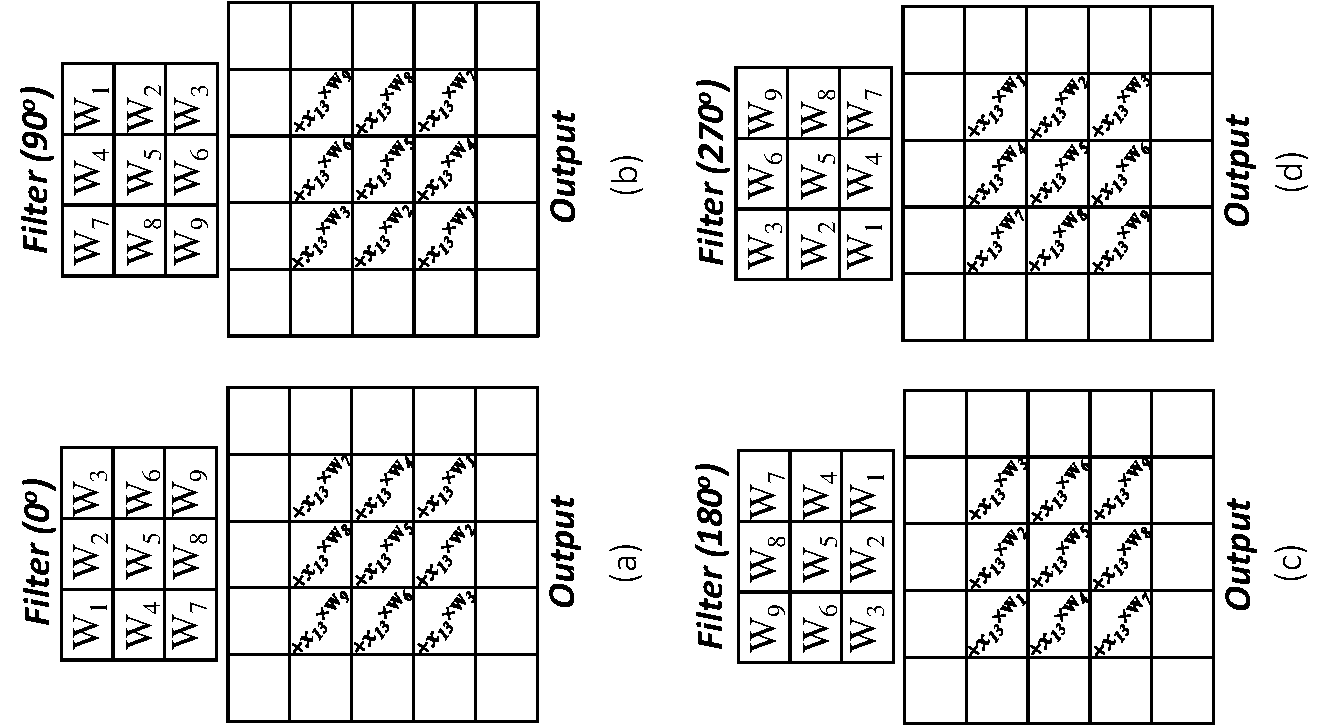
\includegraphics[width=12cm, angle=-90]{fig/method/p4-eps-converted-to.pdf}
\caption{Implementation of $p4$ group convolution with scatter operation where the original filter is rotated (a) $0^\circ$  (b) $90^\circ$  (c) $180^\circ$ (d) $270^\circ$.}
\label{fig:p4}
\end{figure}  

Formally,
for the four symmetric rotations \(r \in \{0,1,2,3\}\), corresponding to 
\(0^\circ, 90^\circ, 180^\circ,\) and \(270^\circ\), let 
\((m',n') = R_r(m,n)\) denote the rotated kernel coordinates obtained by 
applying the spatial rotation operator \(R_r\) to the original offsets 
\((m,n)\). Under this rotation, the scatter-based convolution becomes
\begin{equation}
\label{eq:rot-scatter}
\begin{split}
Y_{c_o,\; i - m' + \lfloor K_h/2\rfloor,\;
               j - n' + \lfloor K_w/2\rfloor}
\; +=\; \\
\sum_{c_i=0}^{C_{\mathrm{in}}-1}
X_{c_i,h,w}\; W_{c_o,c_i,m,n},
\\[6pt]
\substack{
\displaystyle m \in \{0,\dots,K_h-1\},\quad
\displaystyle n \in \{0,\dots,K_w-1\},\\[4pt]
\displaystyle h \in \{0,\dots,H'-1\},\quad
\displaystyle w \in \{0,\dots,W'-1\},\\[4pt]
\displaystyle c_o \in \{0,\dots,C_{\mathrm{out}}-1\},\quad
\displaystyle r \in \{0,1,2,3\}.
}
\end{split}
\end{equation}
In this expression, the channel-wise multiplication and accumulation term 
\(\sum\limits_{c_i=0}^{C_{\mathrm{in}}-1} X_{c_i,h,w}\, W_{c_o,c_i,m,n}\) is computed only once. 
For each rotation \(r\), this accumulated product is added to a different output location 
because the kernel coordinate \((m,n)\) is transformed to its rotated counterpart 
\((m',n') = R_r(m,n)\). Thus, only the scatter location changes across rotations, 
while the channel-wise multiplication and accumulation is reused for all four orientations.

A rotation-invariant response can be obtained by group pooling over the four
orientations. For example, average pooling yields
\begin{equation}
\label{eq:p4-pooling-avg}
\widetilde{Y}_{c_o,h,w}
=
\frac{1}{4}\sum_{r=0}^{3} Y_{c_o,r,h,w}.
\end{equation}
Alternatively, max pooling over orientations may be used:
\begin{equation}
\label{eq:p4-pooling-max}
\widetilde{Y}_{c_o,h,w}
=
\max_{r \in \{0,1,2,3\}} \; Y_{c_o,r,h,w}.
\end{equation}

For symmetric rotation equivariant convolution, the number of filters will increase with the increase of the dimension of the input data. Consequently, the computational overhead also increases. However, with the scatter operation, the multiplication just needs to be performed for one filter and the result of the multiplication can be reused by the other filters directly. It means the number of multiplications is a constant (with respect to the number of directions) and the convolution is only dominated by the addition operation. 

Now we introduce the gradient computation for the rotation-invariant convolution.
During backpropagation, the loss gradient propagates from the output toward the input.
The incoming (upstream) gradient from the next layer is denoted by
\[
G_{c_o,h,w}
=
\frac{\partial\mathcal{L}}{\partial \widetilde{Y}_{c_o,h,w}}.
\]
where \(\widetilde{\mathbf{Y}}\) is the rotation-invariant output feature map obtained after
orientation pooling. 
We derive the gradients with respect to the
rotation-equivariant feature maps \(\mathbf{Y}_{c_o,r,h,w}\),
the input feature maps \(\mathbf{X}\),
and the base convolution kernel \(\mathbf{W}\).


For average pooling, the gradient is distributed equally:
\begin{equation}
\label{eq:rot-back-avg}
\frac{\partial\mathcal{L}}{\partial Y_{c_o,r,h,w}}
=
\frac{1}{4}\,G_{c_o,h,w}.
\end{equation}
For max pooling, we define
\[
r^\star(c_o,h,w)
\in
\arg\max_{r} Y_{c_o,r,h,w}.
\]
Then the gradient passes only through the maximal rotation:
\begin{equation}
\label{eq:rot-back-max}
\frac{\partial\mathcal{L}}{\partial Y_{c_o,r,h,w}}
=
G_{c_o,h,w}\;
\mathbf{1}\!\left[r = r^\star(c_o,h,w)\right].
\end{equation}
Let
\[
\Delta_{c_o,r,h,w}
=
\frac{\partial\mathcal{L}}{\partial Y_{c_o,r,h,w}}
\]
for compactness in the following derivations.


For each rotation \(r \in \{0,1,2,3\}\), the gradients with respect to the
input and the \(r\)-rotated kernel \(\mathbf{W}^{(r)}\)
are given by the standard convolution backward formulas:

\begin{equation}
\label{eq:rot-back-X-explicit}
\frac{\partial\mathcal{L}}{\partial X_{c_i,h,w}}^{(r)}
=
\sum_{c_o=0}^{C_{\mathrm{out}}-1}
\sum_{i=0}^{K_h-1}
\sum_{j=0}^{K_w-1}
W^{(r)}_{c_o,c_i,i,j}\;
\Delta_{c_o,r,\,h-i,\,w-j},
\end{equation}

\begin{equation}
\label{eq:rot-back-W-explicit}
\frac{\partial\mathcal{L}}{\partial W^{(r)}_{c_o,c_i,i,j}}
=
\sum_{h=0}^{H'-1}
\sum_{w=0}^{W'-1}
X_{c_i,\,h+i,\,w+j}\;
\Delta_{c_o,r,h,w}.
\end{equation}


The total gradient with respect to the input feature map is the sum over
the four rotated branches:
\begin{equation}
\label{eq:rot-back-X-total}
\frac{\partial\mathcal{L}}{\partial X_{c_i,h,w}}
=
\sum_{r=0}^{3}
\frac{\partial\mathcal{L}}{\partial X_{c_i,h,w}}^{(r)}.
\end{equation}

To obtain the gradient with respect to the unrotated base kernel
\(\mathbf{W}\),
each rotated kernel gradient is first inverse-rotated
and then accumulated:
\begin{equation}
\label{eq:rot-back-W-total}
\frac{\partial\mathcal{L}}{\partial W_{c_o,c_i,i,j}}
=
\sum_{r=0}^{3}
R_{-r}\!\left(
\frac{\partial\mathcal{L}}{\partial W^{(r)}_{c_o,c_i,i,j}}
\right).
\end{equation}
Here \(R_{-r}\) denotes a rotation of the gradient by \(-r\times90^\circ\),
mapping each rotated kernel’s gradient back to the base orientation.
The proposed scatter approach can also accelerate backpropagation, since the gradient computations themselves are convolution operations, as shown in these formulations.


\subsection{Parallelization of the scatter operation} \label{sec:para}

The parallelization of the convolution with scatter operation is shown in Fig. \ref{fig:PSO}.  In each parallel step, every processor $P_i$ reads the corresponding input data $x_i$ and multiplies it with the same filter weight, then the results of those multiplications will be added to the different output locations. Multiplication with the same filter weight can avoid Write after Write hazard, if there is a synchronization between two parallel steps. For G-convolution, the multiplication is performed only once using this approach.
\begin{figure}[h]
\centering
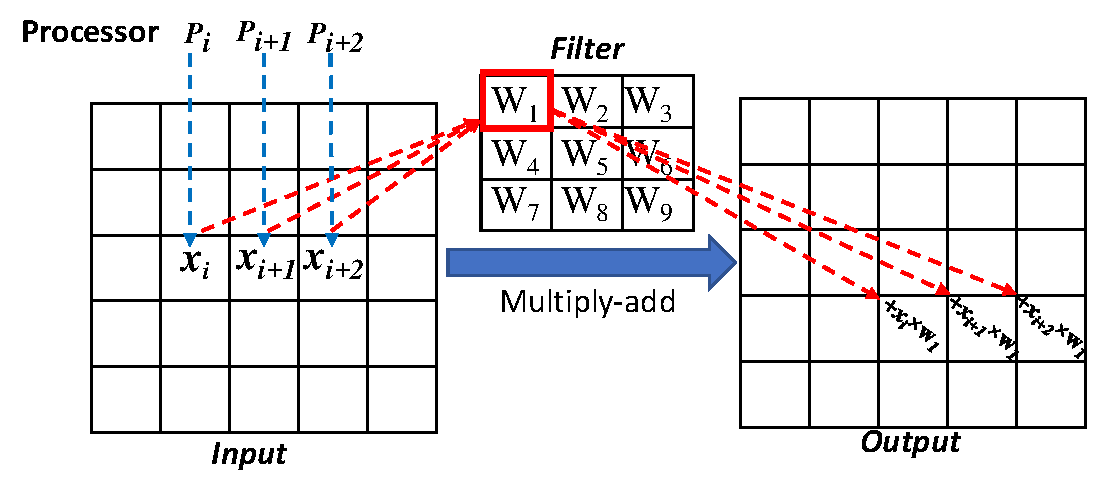
\includegraphics[width=8cm]{fig/method/para-scatter-operation-eps-converted-to.pdf}
\caption{Parallel scatter operation, where each processor $P_i$ corresponds to each input data.}
\label{fig:PSO}
\end{figure}

The scatter operation is a cache friendly operation and can be easily vectorized. As shown in Fig. \ref{fig:cache-cohe}, if all reading positions in the input data are in the same row and are multiplied by the same filter weight, then all writing positions in the output are always in the same row, no matter which filter weight is  multiplied. Even if the filter is rotated symmetrically, all writing positions in the output are also in the same row, see Fig. \ref{fig:cache-cohe-rot}. It meets the data locality requirement of modern SIMD architecture. On the other hand, this figure also shows us a way to reduce the number of synchronizations required. All processors multiply its own input data with the same filter weight and add the result in 4 different outputs. Obviously, before completing the last addition, all processors have no need to be synchronized since they are writing different memory positions of different outputs. We just insert a synchronization after the last addition. The number of synchronizations can be reduced 4 times. 
 
\begin{figure}[h]
\centering
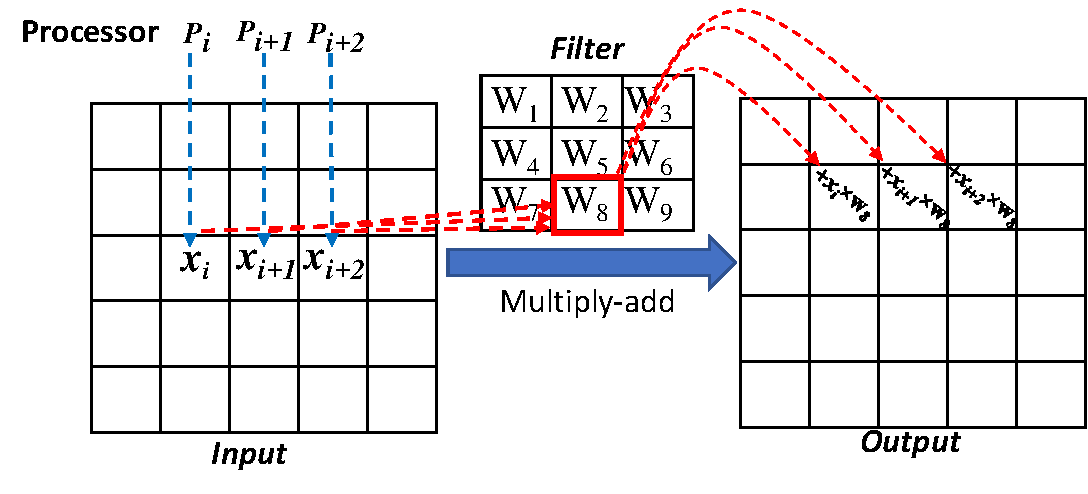
\includegraphics[width=8cm]{fig/method/cache-cohe-eps-converted-to.pdf}
\caption{Illustration of scatter operation by multiplying each input data with another filter weight. No matter which filter weight it is multiplied by, all writing positions in the output are always in the same row.}
\label{fig:cache-cohe}
\end{figure}

\begin{figure}[h]
\centering
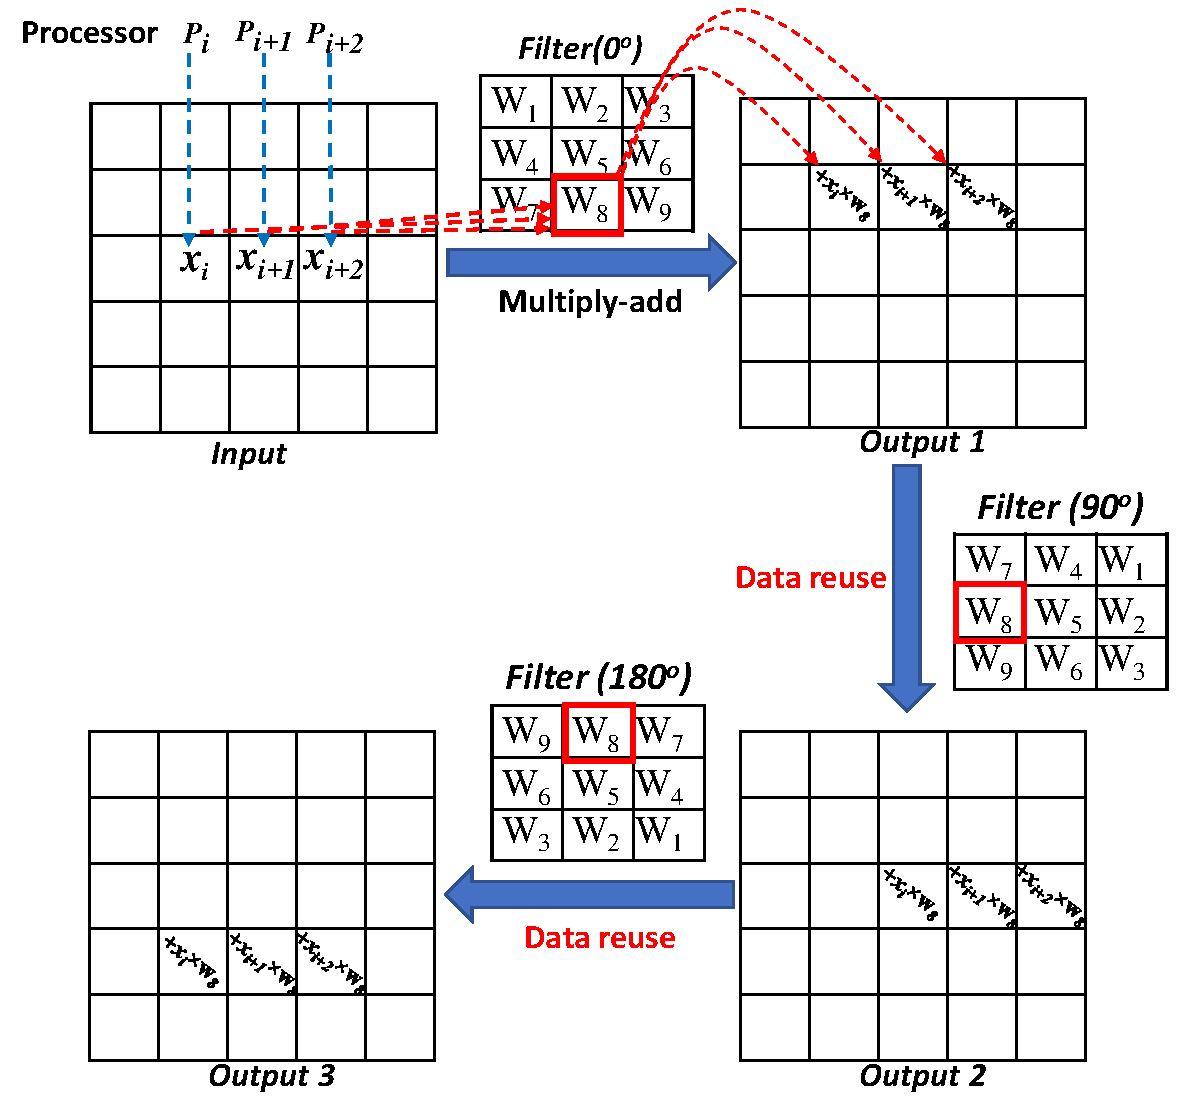
\includegraphics[width=8cm]{fig/method/cache-cohe_rot-eps-converted-to.pdf}
\caption{Output positions for the rotated filter with data reuse. No matter how the filter is rotated, all writing positions in the output are always in the same row if the processors process input data in one row.}
\label{fig:cache-cohe-rot}
\end{figure}


\subsection{Arbitrary rotation convolution formulation} \label{sec:fft_arbitrary}
An interpolation is required for sampling after rotation with arbitrary angle. 
However, it can introduce artifacts that degrade the performance of rotation-invariant models.
%In addition, the interpolation is an expensive operation, especially for some interpolations such as bicubic interpolation. 
In this subsection, we propose an approach which takes the advantage of symmetric rotation and steerable filter to implement rotation-invariant convolution with filter arbitrarily rotated. 
The proposed method accelerates the training process while eliminating the need for interpolation.
\begin{figure}[ht]
\begin{center}
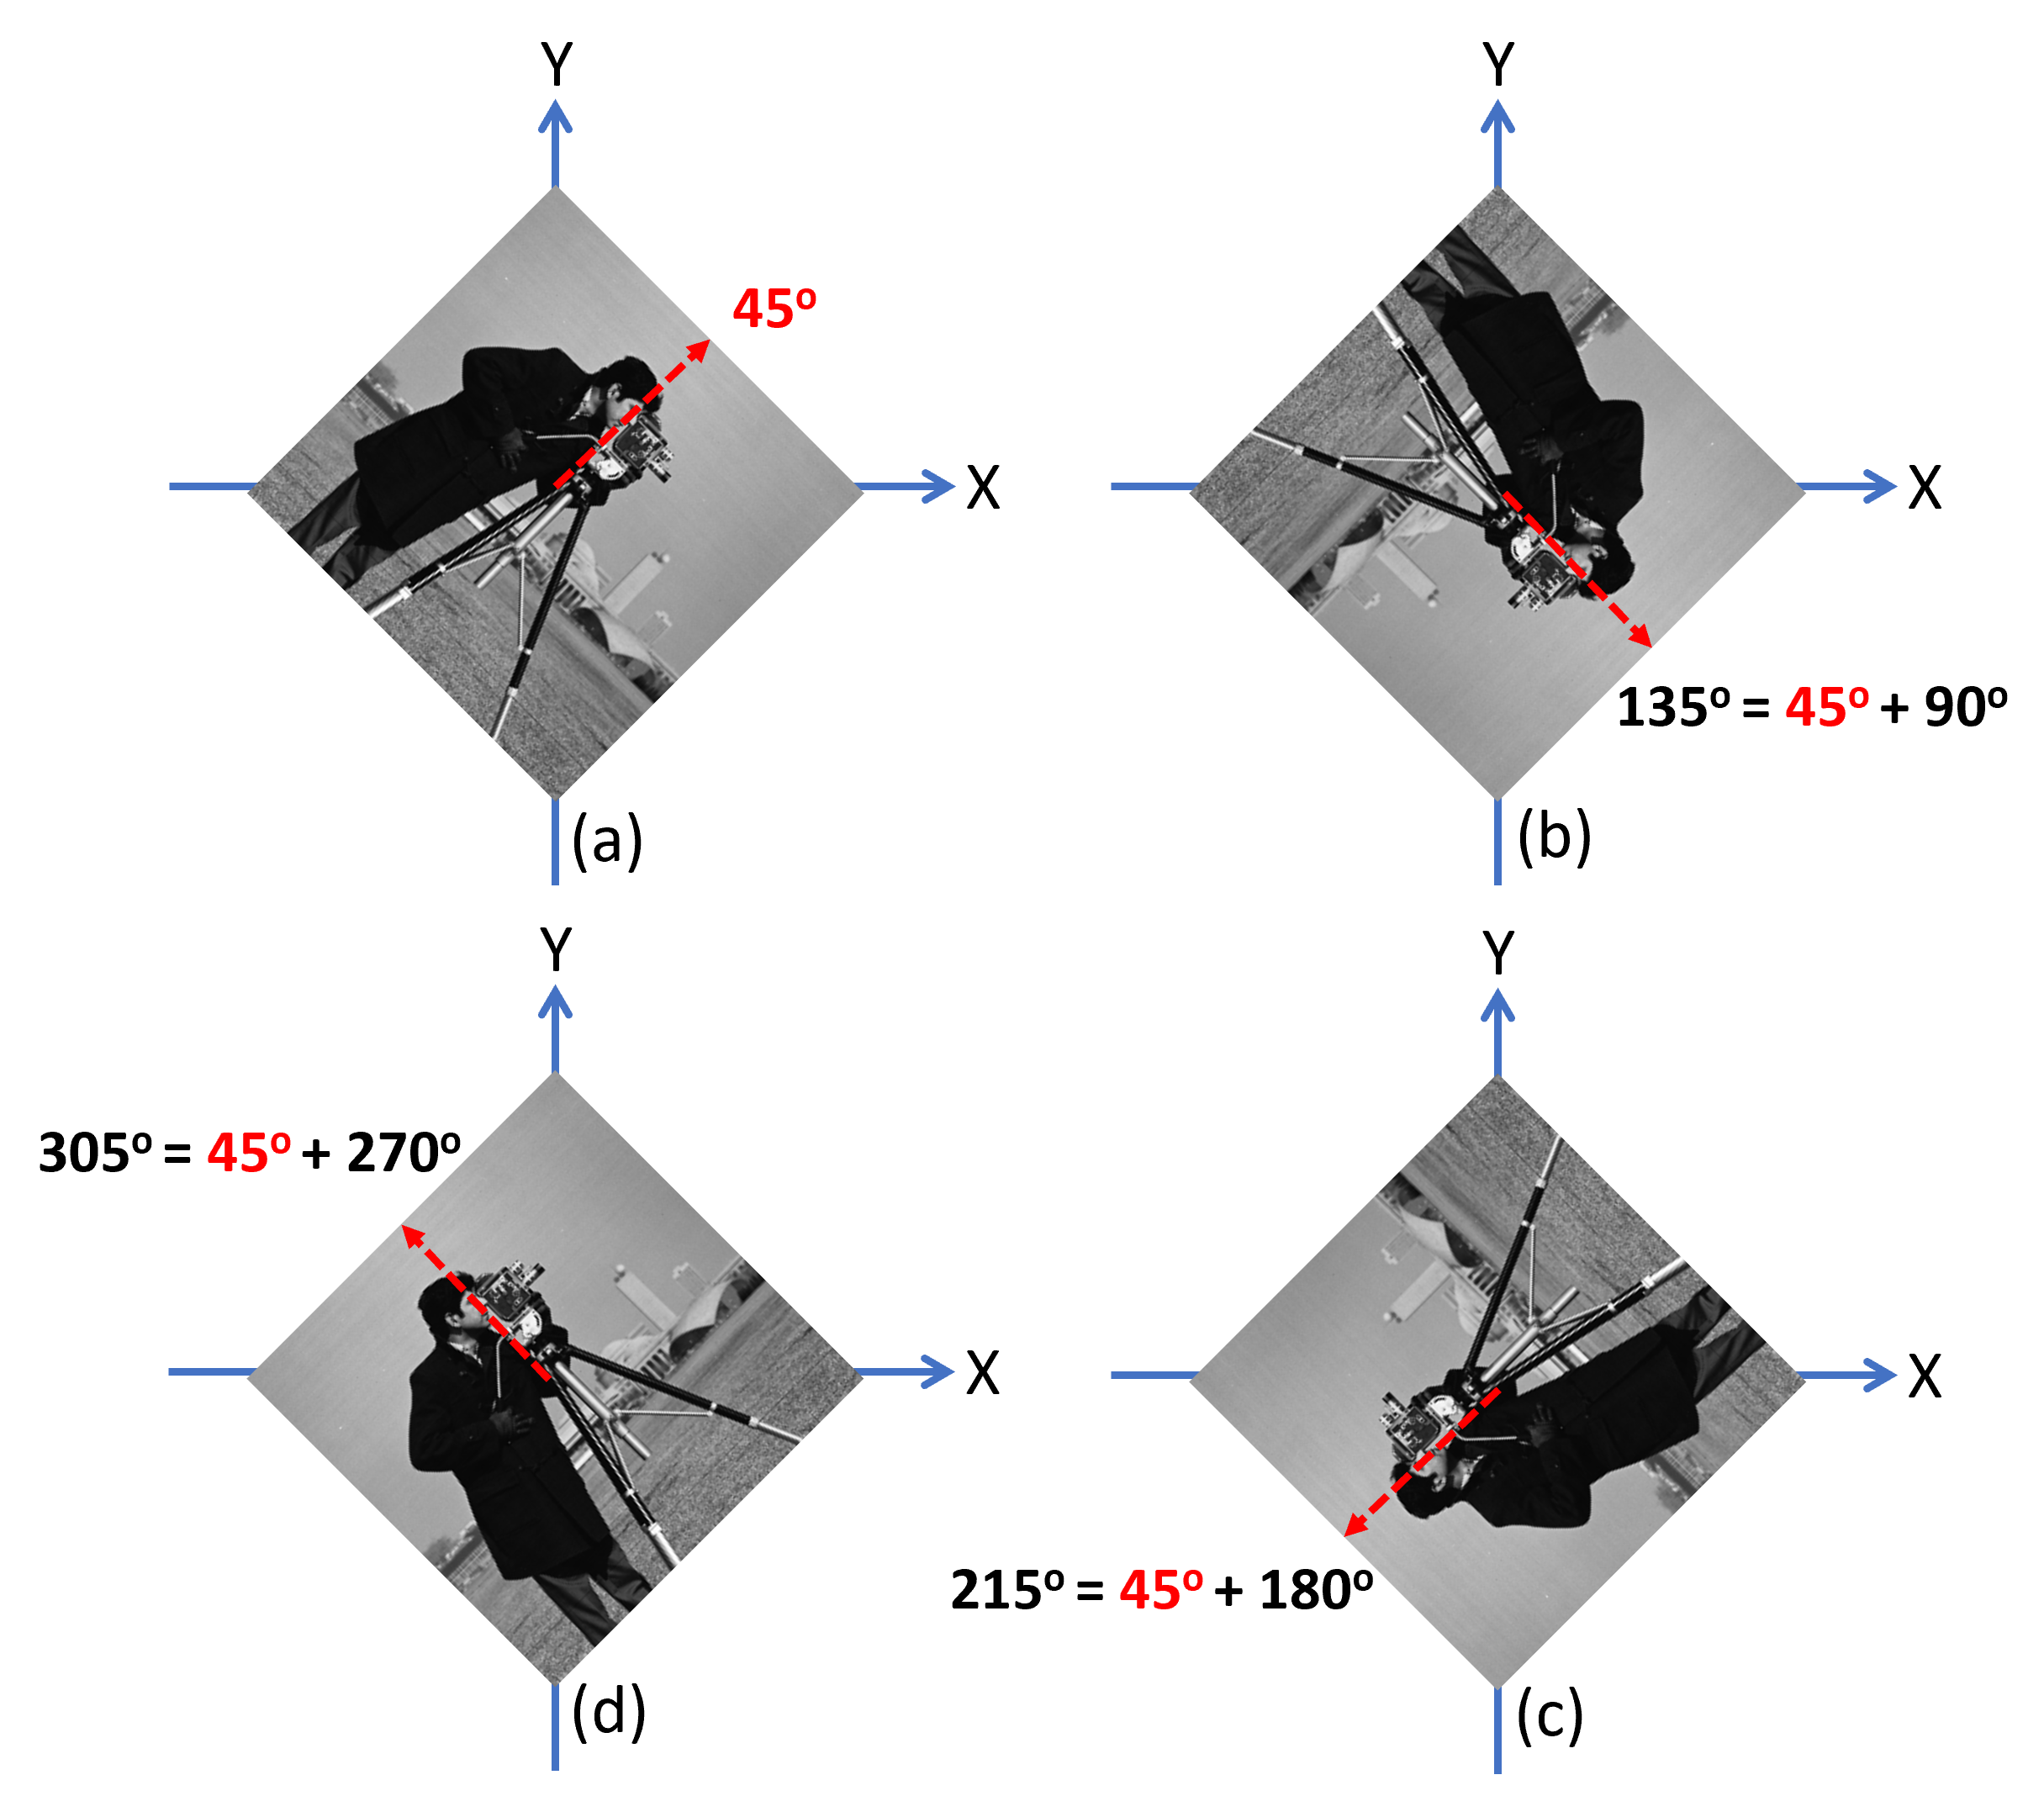
\includegraphics[scale=0.44]{fig/method/quadrant.png}
\caption{Symmetric correspondents of $45^\circ$ rotated image in other quadrants of coordinate plane}
\label{fig:quadrant}
\end{center}
\end{figure}


The sampled orientations are usually evenly distributed in rotation space for rotation equivariance convolution. For example, the angle increment between every two successive rotations is $\frac{\pi}{12}$, if the number of sampled orientations is 24. We observe the rotation angle in the first quadrant of coordinate plane always has a symmetric correspondent in each of other quadrants, see Fig. \ref{fig:quadrant}. As shown in the figure, the rotated versions of image with angles $135^\circ$, $215^\circ$ and $305^\circ$ can be obtained by symmetrically rotating the $45^\circ$-rotated image by $90^\circ$, $180^\circ$ and $270^\circ$, respectively.    
This observation gives us a chance to accelerate the rotation equivariance convolution with filter arbitrarily rotated. We apply filter rotations when the rotation angle falls within the first quadrant. Rotations in other quadrants can be obtained by symmetrically mapping the correspondence from the first quadrant. The number of rotations is reduced by 75$\%$. This indicate that we can rotate the filter in the first quadrant of coordinate plane, and perform the multiplication for the rotations in the first quadrant. We then reuse these multiplication results for the rotation in the other quadrants. 

As steerable filters can generate rotated responses without relying on interpolation,  
we construct the filter in the first quadrant of the coordinate plane using the following steerable filter formulation as in \cite{93808}:
\begin{equation}
\psi_\theta(x, y) = \sin(\theta) \cdot f_x(x, y) + \cos(\theta) \cdot f_y(x, y)
\label{eq:steerable_filter}
\end{equation}
Equation~\eqref{eq:steerable_filter} defines the steerable filter \( \psi_\theta(x, y) \) at a given rotation angle \( \theta \),  
where \( (x, y) \in \mathbb{R}^2 \) denotes the spatial coordinates.
The functions \( f_x(x, y) \) and \( f_y(x, y) \) represent the learned base filters oriented along the horizontal (x-axis)  
and vertical (y-axis) directions, respectively. The steerable filter \( \psi_\theta(x, y) \) is constructed as a linear combination  
of these directional basis filters using fixed orientation-dependent coefficients \( \sin(\theta) \) and \( \cos(\theta) \),  
enabling efficient and continuous steering of the filter to any desired angle \( \theta \).

To encourage the learned base filters to exhibit steerable behavior, we add two regularization losses to the standard
cross-entropy objective. The overall loss is defined as:
\begin{equation}
\mathcal{L}_{\text{total}}
=
\mathcal{L}_{\text{CE}}
+
\lambda_{\text{mag}}\,\mathcal{L}_{\text{mag}}
+
\lambda_{\text{orth}}\,\mathcal{L}_{\text{orth}} ,
\label{eq:total_loss}
\end{equation}
where \( \mathcal{L}_{\text{CE}} \) denotes the task-specific cross-entropy loss,
and \( \lambda_{\text{mag}} \) and \( \lambda_{\text{orth}} \) are scalar weighting coefficients controlling
the strength of the magnitude and orthogonality regularizations, respectively.

The magnitude-matching loss encourages the two base filters to maintain similar energy levels:
\begin{equation}
\mathcal{L}_{\text{mag}}
=
\frac{1}{B}
\sum_{b=1}^{B}
\left(
\left\|\mathbf{w}^{(x)}_{b}\right\|_{2}
-
\left\|\mathbf{w}^{(y)}_{b}\right\|_{2}
\right)^{2},
\label{eq:mag_loss}
\end{equation}
where \( \mathbf{w}^{(x)}_{b} \) and \( \mathbf{w}^{(y)}_{b} \) denote the flattened kernel weights associated with 
the \( b \)-th filter in the base filters \( f_x \) and \( f_y \), respectively, and \( B \) is the total number of filters.



The orthogonality loss penalizes the correlation between the two directional bases, promoting rotational independence:
\begin{equation}
\mathcal{L}_{\text{orth}}
=
\frac{1}{B}
\sum_{b=1}^{B}
\left(
\frac{
\left\langle \mathbf{w}^{(x)}_{b}, \mathbf{w}^{(y)}_{b} \right\rangle
}{
\left\|\mathbf{w}^{(x)}_{b}\right\|_{2}
\left\|\mathbf{w}^{(y)}_{b}\right\|_{2}
+ \varepsilon
}
\right)^{2},
\label{eq:orth_loss}
\end{equation}
where \( \varepsilon \!>\! 0 \) ensures numerical stability during training.
Together, these regularization terms guide the base filters \( f_x \) and \( f_y \)
toward forming an approximately steerable pair that preserves orientation consistency across rotations.


\section{GPU implementation}\label{sec:GPU}

%Graphics Processing Units (GPUs) are the main hardware for the acceleration of modern CNNs. 
%We aim our implementation on CUDA-enabled GPUs where CUDA (Compute Unified Device Architecture) is a parallel computing 
%platform and application programming interface developed by NVIDIA.
\subsection{GPU implementation of single-orientation convolution with scatter operation}\label{sec:GPU}
The convolution operation can be efficiently implemented on GPU using matrix multiplication, as shown in \cite{cudnn-arxiv}. This approach requires transforming the input image and the convolution kernel into matrices that can exploit the fast multiplication capabilities of the GPU. This transformation involves duplicating the input data to lower its dimensionality. 

In our GPU implementation of convolution with scatter operation, we use matrix multiplication to perform the channel-wise multiplication and summation of the input and a filter kernel. To achieve a higher performance,
NVIDIA cuBLAS library  \cite{cublas}, a library of highly optimized matrix multiplication routines, is used to perform the channel-wise multiplication and summation. The results are then scattered to the corresponding output positions according to the scattering rule. Unlike the method in \cite{cudnn-arxiv}, we do not apply any data lowering in our GPU implementation. Our GPU implementation follows gather-GEMM-scatter dataflow \cite{torchsparse} but gather without data lowering. 

Considering that cuBLAS accesses matrices in column-major order, we arrange the input image in CNHW layout and the filter in NHWC layout, as shown in Fig. \ref{fig:mem-layout}. The resulting matrix ensures coalesced access for the parallel implementation of the scatter operation, as described in Section \ref{sec:para}.
\begin{figure}[h]
\centering
    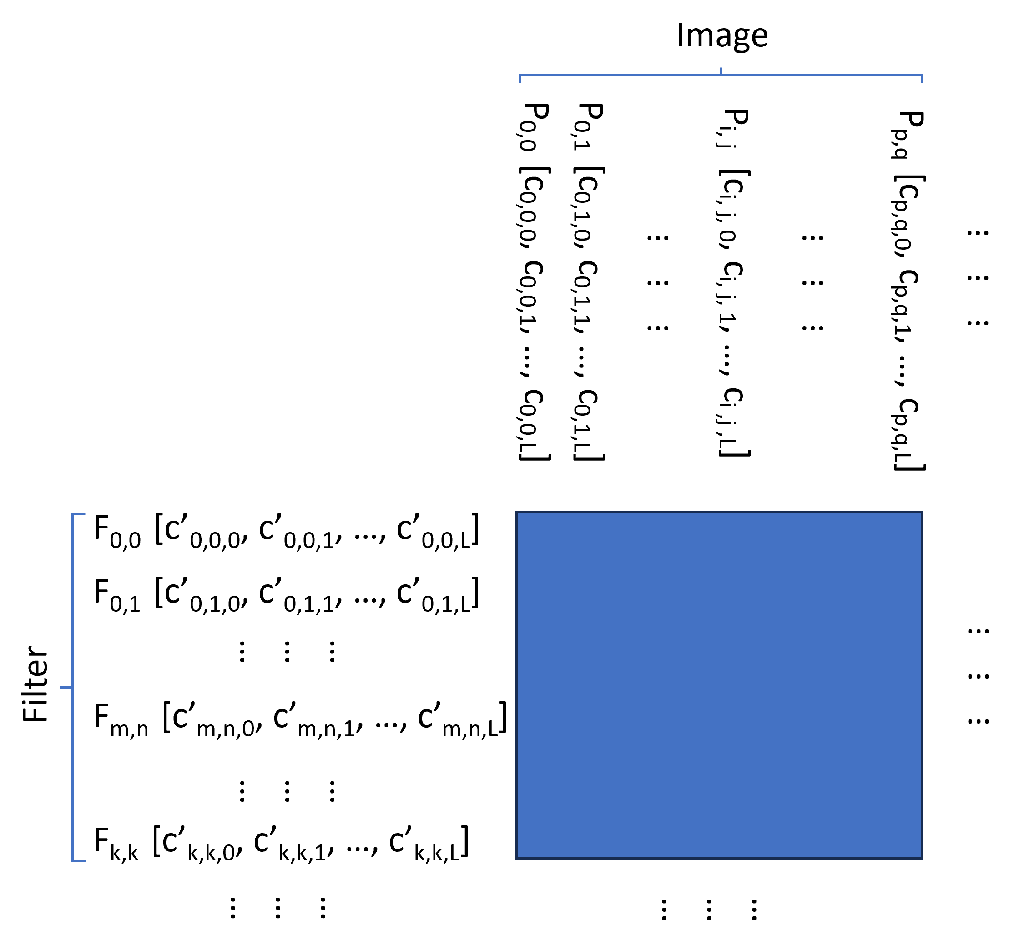
\includegraphics[width=8.5cm]{fig/method/mem-layout.pdf}
\caption{Memory layout of the input image and filter kernel for matrix multiplication, where $P_{i,j}$ represents an image pixel,  $F_{m,n}$ represents an element of the filter kernel, $c_{i,j,L}$ and $c'_{m,n,L}$ are channel values. Only a single image and a single filter are depicted.} 
\label{fig:mem-layout}
\end{figure}


After performing matrix multiplication, the results need to be added to the output image using the parallel scattering operation. However, directly writing to off-chip memory (i.e., the global memory of CUDA) is time-consuming, as each element of the output image needs to be accessed $k^2$ times. To avoid this, we tile the output image as in Fig. \ref{fig:imge-tile} so that each tile can be accommodated in on-chip memory (i.e., the shared memory of CUDA). The scatter operation will be performed in on-chip memory, and the results will then be written to off-chip memory. There is an overlapping region between adjacent tiles, which ensures that elements on the borders can be scattered to neighboring positions completely.
\begin{figure}[h]
\centering
    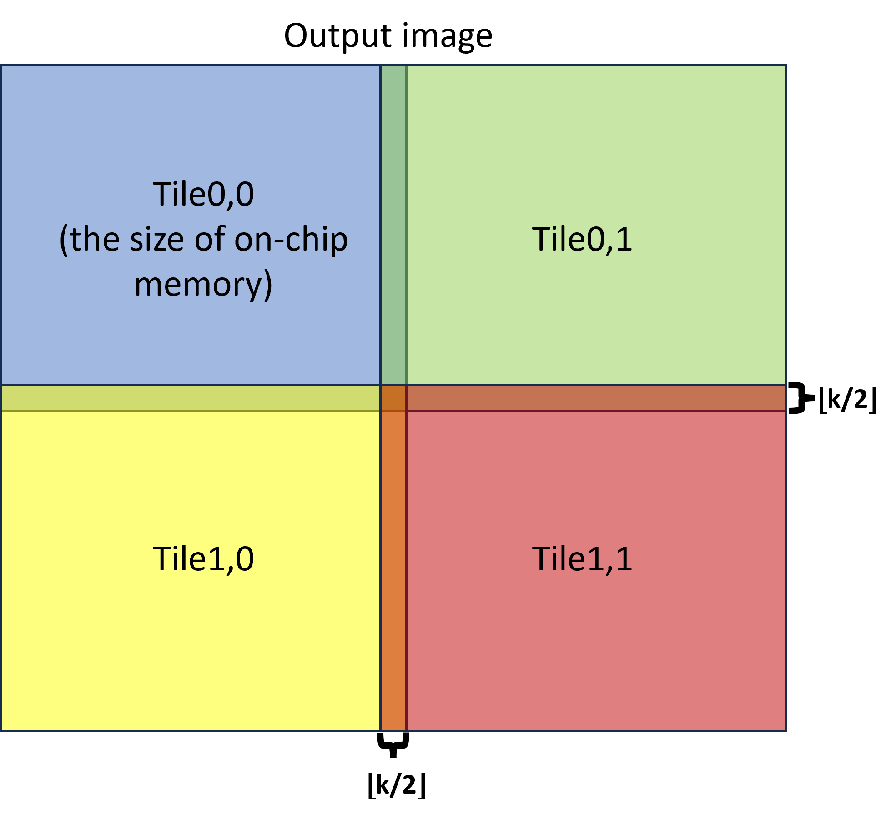
\includegraphics[width=5.5cm]{fig/method/image-tile.pdf}
\caption{Image tiling with on-chip memory of GPU, where the size of overlap between tiles is $\floor {k /2}$.} 
\vspace{-0.4cm}
\label{fig:imge-tile}
\end{figure}

\subsection{GPU implementation of symmetric rotation invariant convolution with scatter operation}\label{sec:GPU}
The main idea behind accelerating symmetric rotation invariant convolution using the scatter operation is the reuse of intermediate multiplication results, as described in Section \ref{subsec:accSymRot}. The matrix-multiplication outputs are shared across all rotations, eliminating redundant computation.
To make the layer rotation invariant, an orientation-pooling operation is applied afterward, which can be implemented in two ways: point-wise average pooling or point-wise max pooling.

For point-wise average pooling, each element in the result of the matrix multiplication is divided by $r$, the number of rotations, before being added to the output image. This means that the required on-chip memory size is equal to the tile size. However, for point-wise max pooling, the on-chip memory must be twice the tile size—one part for computing the current tile and another for storing the previous maximum values. After finishing additions for the current tile, the point-wise max operation is performed between the current tile and the previously stored max tile. This is necessary because max pooling is a non-linear operation, meaning the maximum value cannot be determined before the additions are completed. Additionally, the overlapping region between adjacent tiles must be extended to $\floor {k /2} + 1$ to ensure correct max pooling calculations.  Only the central part of each tile, excluding $\floor {k /2} + 1$ border lines, is used in the final output. This ensures that the max values are computed correctly without missing contributions from neighboring tiles.

